\section{Beyond Parameters: Executable Native System Design}
\label{sec:native-design}

We treat design freedom and optimization method as separate axes. Parameters,
implementation code, typed protocols, graph wiring and execution order are
successively broader design variables; black-box, gradient and hybrid methods
are ways to propose them. Differentiability must not force the science world
into a simpler ontology. The original researcher world is a minimum contained
instance, not the ceiling of future scientific activity.

\subsection{Executable code, communication and graph edits}

The opt-in native kernel runs a \systemspec{} graph around the actual
\suto{} lifecycle. A four-year Qwen3-8B integration probe with five independent
researchers completed 147 model requests and delivered 20 institutional
messages. Saved HTTP inputs establish that new context reached subsequent
researcher calls. This demonstrates delivery, not a causal scientific benefit:
there was no paired no-institution live comparison.

A separate restartable black-box campaign exercises one joint transaction:
after observing baseline loss, it adds a Python producer, a new deliberation
protocol and two edges, replaces selection with a Python consumer, and places
the producer before selection. Both code implementations execute four times
and affect real submitted-paper decisions. The proposer is developer-authored;
its threshold depends on the previous observation. Negative accepted-decision
count changes from $-4$ to $-2$, so the baseline remains incumbent. The edit is
technically valid but worse under the declared loss. No hidden policy veto or
fabricated failure penalty is involved.

\subsection{One institution, hard and soft execution}

Native tensor programs give the same represented institution operational hard
and relaxed interpretations: discrete versus soft addressing, gates and
branches, with explicit tensor state and memory. In the live probe, a Python
producer extracts actual review features; query/key addressing selects
threshold slots; a gate produces decisions; a Python consumer commits them to
native publication. Research, retrieval and researcher decisions are not
replaced with numeric production equations.

Let $\bar z$ denote opaque observations collected from the initial native run,
$T_\theta^{\mathrm{soft}}$ the represented institutional computation, and
$\ell$ the declared conditional objective. The optimized derivative is
\begin{equation}
 \nabla_\theta\widetilde L(\theta;\bar z)
 =\nabla_\theta\ell\bigl(T_\theta^{\mathrm{soft}}(\bar z)\bigr),
 \qquad \bar z\ \text{held fixed}.
\end{equation}
This is not the derivative of the expected full native-world loss
$L(S(\theta))$. Autograd can traverse represented tensor institutions, tensor
edges and memory; it does not yet traverse arbitrary Python, retrieval or the
LLM's response to changed inputs. Holding the LLM weights fixed is appropriate,
but does not make researcher responses constant as institutions change.

The initial institution is developer-authored. Thirty Adam steps fit seven
coordinates (four keys, two threshold slots and one bias; learning rate 0.1,
temperature 0.8) on its real native trace. Conditional negative soft
accepted-count changes from $-0.48291$ to $-2.96997$. The fitted hard program
is then installed into a fresh original-world execution with the same fixed
model, corpus and seed. Actual loss changes from $0$ to $-3$
(Figure~\ref{fig:native-gradient}). Seven real-trace central differences agree
with autograd to maximum absolute error $6.53\times10^{-11}$; the complete fit
path and installed program independently reproduce. This tests the represented
derivative, not the missing full-world derivative.

\begin{figure}[ht]
 \centering
 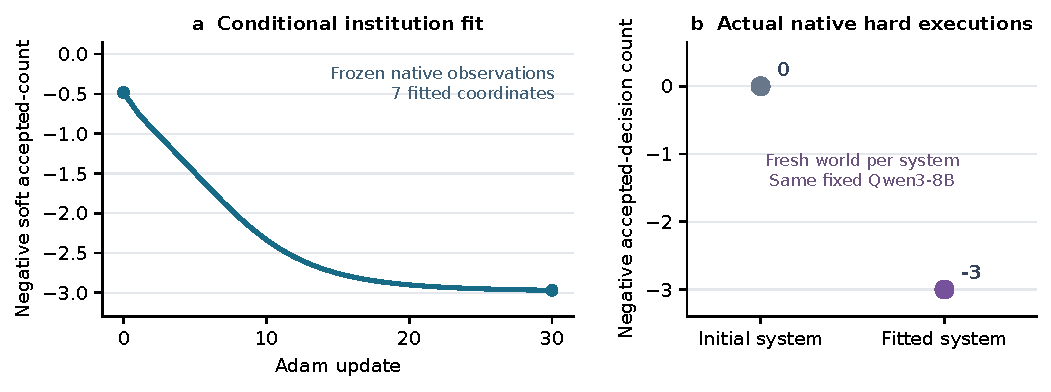
\includegraphics[width=\linewidth]{figures/native-design-evidence.pdf}
 \caption{Separate evidence layers in the native hard/soft probe. Left: the
 recorded conditional fitting path on frozen native observations. Right:
 actual hard executions of the initial and fitted institutions in two fresh
 native worlds. These are not points on one common loss trajectory. The
 accepted-count target permits all-accept; lower loss is not better science.
 One development seed (1301), five researchers and two years per system; no
 held-out or uncertainty claim.}
 \label{fig:native-gradient}
\end{figure}

\subsection{Model-written source: execution is not invention success}

Qwen3-8B generated a Python \code{step(context)} institution named Peer
Observer. The exact source passed three isolated probes on actual native
snapshots and ran twice in a fresh two-year world. Its condition (more than
three paper records for an author) never fired: zero messages were emitted or
delivered. Thus native source execution succeeded, but no researcher-input
effect or useful institutional behavior was observed. The host supplied the
observation/delivery attachment and compiled a prose protocol description to
a stable artifact ID; this is not model-invented topology. Nine earlier
proposal/metadata failures remain recorded with no invented losses.

\begin{table}[ht]
\caption{Distinct native development probes. Timings cover completed drivers
after preflight, not total debugging or isolated inference throughput. All use
fixed Qwen3-8B weights and five researchers; none is held-out policy evidence.}
\label{tab:native-probes}
\centering\small
\begin{tabular}{p{0.22\linewidth}cp{0.44\linewidth}r}
\toprule
Probe & Years/system & Observed result & Seconds \\
\midrule
Context integration & 4 & 20 delivered messages; no paired benefit test & 532.27 \\
Joint source/graph edit & 4 & Loss $-4\to-2$; original retained & 1,077.93 \\
Conditional hard/soft fit & 2 & Native loss $0\to-3$; all-accept legal & 488.63 \\
Generated source & 2 & Two executions, zero messages; inert trigger & 167.25 \\
\bottomrule
\end{tabular}
\end{table}

The joint-edit, gradient-fit and source-only probes start from different
institutions and protocols; their absolute losses are not a method leaderboard.
The gradient probe uses 111 model responses across two worlds; the joint edit
uses 302; the source execution uses 56. A separate numeric miniature has
complete relaxed recurrent-world autograd; it is not evidence of full
original-world backpropagation. Later development integrations below close
execution gaps without presuming beneficial institutional discovery.

\subsection{Actual-feedback source revision: a negative result}

The new source proposer restores real native checkpoints and supplies prior
losses, author state, mechanism activity, delivered messages and, in amended
probes, bounded actual paper histories. It records the exact proposed source,
history/loss bindings, isolated execution and subsequent fresh native score.
Ports and host attachment remain fixed on this source-only route; separate
atomic graph patches support broader edits. There is no message-count reward,
activity floor or hand-written replacement of an inert valid program.

Two initial-plus-two-revision loops each observe losses $[-1,-1,-1]$ over
two-year worlds. Adding explicit diagnosis-before-code and a preregistered
three-year horizon gives $[-2,-2]$ (Table~\ref{tab:native-feedback}). All five
executed revisions return the same source bytes and deliver zero messages.
Rationales sometimes describe an algorithm change absent from the code.
The planned route first generates an altered algorithm but accesses a missing
top-level paper decision; its one isolated technical repair restores the inert
trigger. These failed drafts are retained, not assigned fabricated losses.
The horizon amendment allows year2 papers to affect year3 research, not a
matched comparison against the shorter probes. The result demonstrates a
working result-conditioned source loop, not useful institutional invention.

\begin{table}[ht]
\caption{New native feedback probes, development seed1301. Systems are fresh
executions; settings differ, so absolute losses are not a method leaderboard.
Driver times exclude preflight. Fixed Qwen3-8B and five researchers throughout.}
\label{tab:native-feedback}
\centering\small
\begin{tabular}{p{0.37\linewidth}ccr}
\toprule
Probe & Years / systems & Native losses & Seconds \\
\midrule
Loss/activity source feedback & 2 / 3 & $-1,-1,-1$ & 568.37 \\
Add real paper records & 2 / 3 & $-1,-1,-1$ & 575.02 \\
Plan then code, longer horizon & 3 / 2 & $-2,-2$ & 758.71 \\
Antithetic full-native costs & 2 / 2 & $-1,-1$ & 362.14 \\
\bottomrule
\end{tabular}
\end{table}

\subsection{Full-native cost gradients without pathwise world backpropagation}

The distribution-gradient route now has a live probe, distinct from conditional
tensor fitting. Let $z$ be latent design coordinates, $S(z)$ their bounded
SystemSpec mapping, and $L$ the complete native cost. Antithetic draws estimate
\begin{equation}
 \nabla_\mu\,\mathbb{E}_{\epsilon,\xi}
 L\bigl(S(\mu+\sigma\epsilon),\xi\bigr)
 \ \approx\ \frac{1}{m}\sum_{i=1}^m
 \frac{L_i^+-L_i^-}{2\sigma}\,\epsilon_i,
 \qquad \epsilon_i\sim\mathcal{N}(0,I).
\end{equation}
Each cost reruns the original native world, including changed fixed-LLM
responses, rather than holding observed researcher inputs fixed. No pathwise
input-response Jacobian or whole-world backpropagation is supplied by this
estimator.

One declared developer-authored exploration-advice coordinate uses a single
pair (search seed42, $\sigma=0.7$, learning rate0.1). Both worlds deliver ten
messages; six second-year HTTP requests per world contain the new context,
with request hashes matched to completed response journals. Both costs equal
$-1$, so the gradient is exactly zero and the distribution mean does not move.
No reroll seeks a nonzero result. This proves the cost pathway includes actual
downstream researcher inputs, not that the true derivative is zero or that
gradient optimization improves science. Useful source/graph invention, faithful
full-input differentiation, richer workflows, live-world migration and recursive
designer improvement remain open.
